An extensive Phase-2 upgrade program is also scheduled for CMS Level-1 Trigger~\cite{l1_tdr}. Since RPC is the only Muon detector present in both CMS Barrel and Endcap region, its contribution to CMS Level-1 Trigger upgrade program is important. 

\begin{wrapfigure}[14]{R}{0.6\textwidth}
    \caption{\footnotesize RPC readout and control system for Phase-2. Its links will be composed by Slow Control/Monitoring channels (dashed lines) and readout channels (solid lines). }
    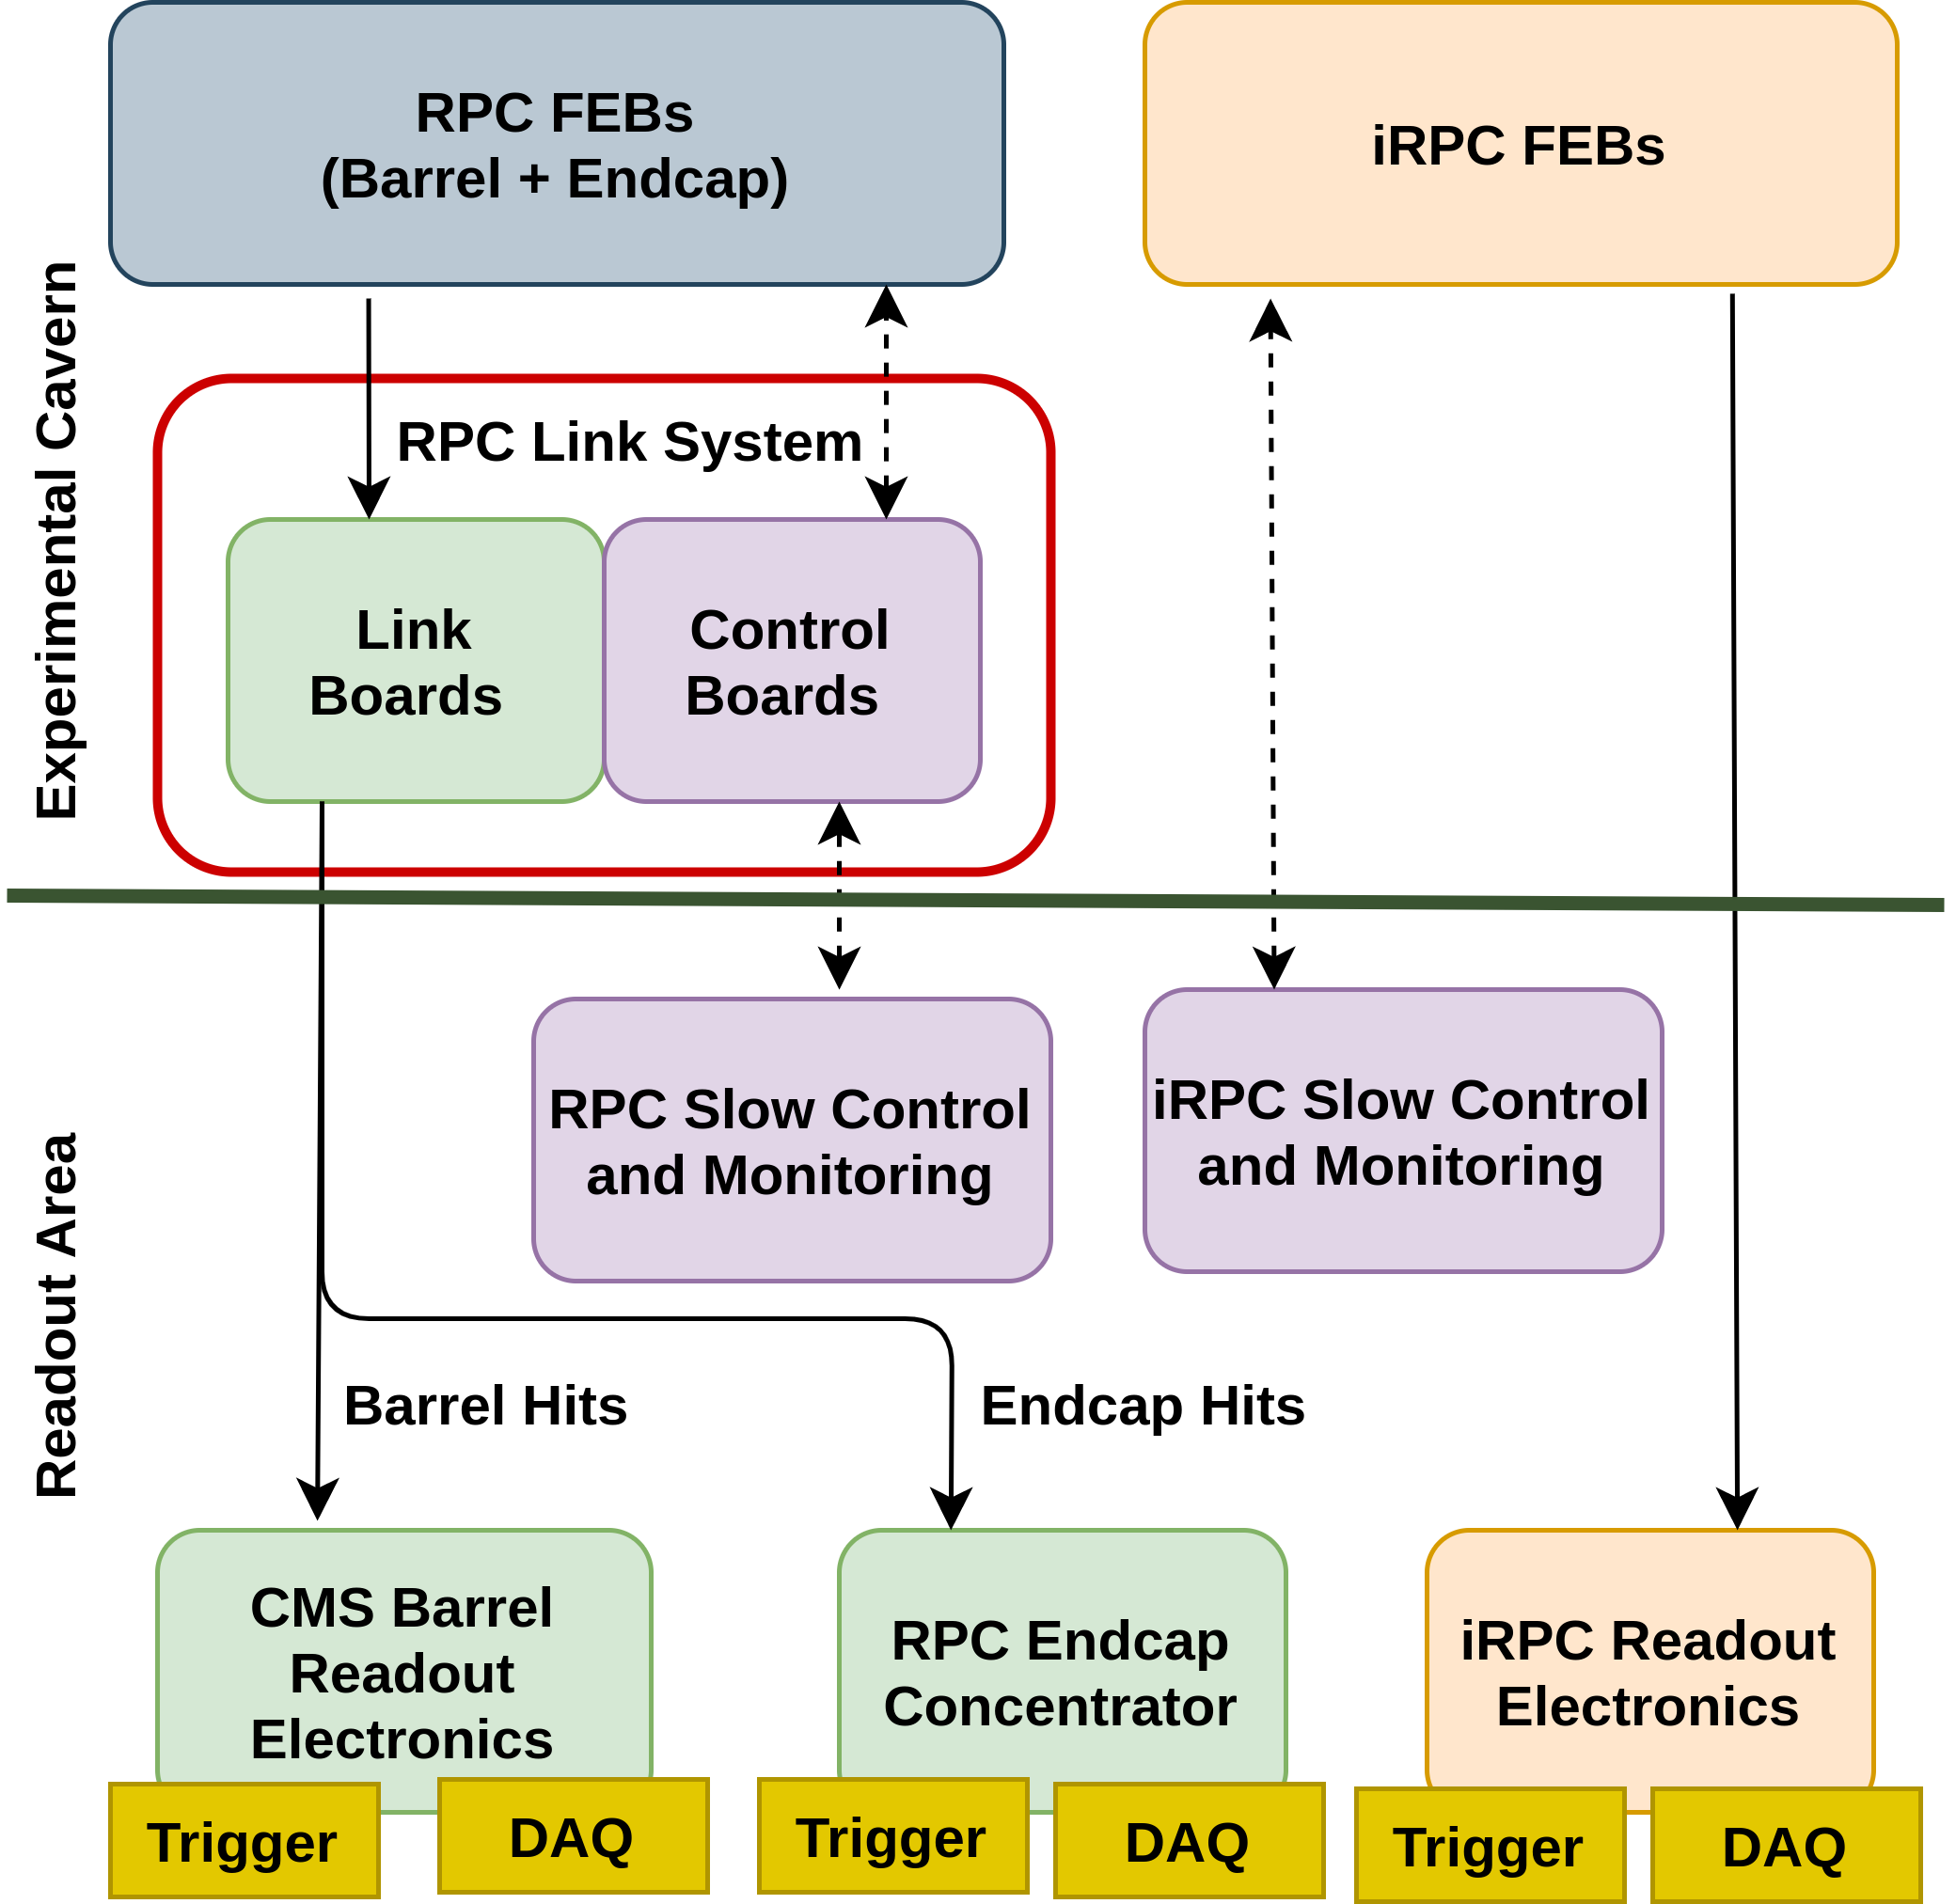
\includegraphics[width=0.6\textwidth]{uioposter-images/rpc_phase2_readout.png}
    \label{rpc_phase2_readout}
\end{wrapfigure}

The readout and control system (also called back-end) of the RPC (Figure 4) system will be redesigned in order to 

% \begin{tcolorbox}[colback=gray!5,colframe=gray!40!black]
%     \textbf{(1) include readout and control of new hardware; (2) cope with the requirements of the Level-1 Trigger Phase-2 design; (3) sustain maintainability of the system by replacing obsolete hardware.}
% \end{tcolorbox}

\begin{tcolorbox}[colback=gray!5,colframe=gray!40!black]
    The readout and control system (also called back-end) of the RPC system will be redesigned in order to:
    \begin{itemize}
        \item include include readout and control of new hardware;
        \item cope with the requirements of the CMS Level-1 Trigger Phase-2 design;
        \item sustain maintenability of the system by replacing obsolete hardware.
    \end{itemize}
\end{tcolorbox}

The new readout, control and monitoring hardware will be installed in the CMS Services Area, away from CMS radiation, and will follow the CMS specification of common hardware platforms for Phase-2, specifically, Serenity boards~\cite{serenity}, with ATCA form factor. 



\begin{tcolorbox}[colback=gray!5,colframe=gray!40!black]
    Barrel RPC hits are expected to be distributed to a common CMS Barrel (RPC + DT) hardware, while Endcap and iRPC hits will go to dedicated RPC boards. Those hits will later be distributed to CMS Muon Track Finders and DAQ.
\end{tcolorbox}

% Different firmwares are expected for the New Link System $\Leftrightarrow$ back-end and iRPC FEB $\Leftrightarrow$ back-end. 